\documentclass{article}

\usepackage[brazil]{babel}
\usepackage[T1]{fontenc}
\usepackage[a4paper, margin=1.5cm]{geometry}
\usepackage[colorlinks, urlcolor=blue, citecolor=red]{hyperref}
\usepackage[utf8]{inputenc}
\usepackage[pdftex]{graphicx}
\usepackage{amsfonts, amsmath, enumitem, float, subcaption}

\title{\textbf{A função \emph{hash} criptográfica SHA-3}}
\author{Gustavo Zambonin\thanks{\texttt{gustavo.zambonin@grad.ufsc.br} ---
todos os algoritmos utilizados podem ser encontrados
também \href{https://github.com/zambonin/ufsc-ine5429}{neste repositório}.} \\
\small {Segurança em Computação (UFSC -- INE5429)} \vspace{-5mm}}
\date{}

\begin{document}

\maketitle

\section{Definições}

\begin{itemize}

\item Uma \emph{função hash criptográfica}, ou função de resumo criptográfica
(futuramente denotada por $h$), é um algoritmo matemático que mapeia uma
quantidade de bytes qualquer\footnote{algumas funções desse tipo têm
limites quanto ao tamanho da entrada, embora estes sejam extremamente
grandes.} para uma palavra de tamanho fixo, ou seja,
$h : \{0, 1\}^{*} \longrightarrow \{0, 1\}^{n}$, $n \in \mathbb{N}$.

Para que seja resistente a diversos tipos de criptoanálise, uma função
$h : X \longrightarrow Y$ deve respeitar algumas propriedades:

\begin{enumerate}[label=\roman*.]

\item \emph{Resistência à pré-imagem}: Para um resumo $M' \in Y$, é
computacionalmente impraticável\footnote{o tempo ou recursos gastos para esta
computação excedem a validade ou utilidade da informação desejada.} encontrar a
mensagem $M \in X$ tal que $h(M) = M'$. Uma função matemática com esta
propriedade é chamada de unidirecional.

\item \emph{Resistência à segunda pré-imagem}: Para uma mensagem $M_0 \in X$,
é computacionalmente impraticável encontrar uma segunda mensagem $M_1 \in X$
tal que $M_0 \neq M_1$ e $h(M_0) = h(M_1)$.

\item \emph{Resistência à colisão}: Para duas mensagens $M_0, M_1 \in X$, é
computacionalmente impraticável encontrar $M_0 \neq M_1$ e $h(M_0) = h(M_1)$.

\end{enumerate}

É importante notar que, embora as definições sejam extremamente parecidas,
resistência à segunda pré-imagem e resistência à colisão são conceitos
diferentes; um atacante não consegue escolher a primeira mensagem caso queira
atacar a resistência à segunda pré-imagem; para a resistência à colisão, o
atacante pode escolher livremente o par de mensagens.

\item Algumas aplicações destas funções são enumeradas abaixo:

\begin{itemize}

\item Podem ser utilizadas para verificar a integridade da mensagem, comparando
resumos criptográficos calculados antes e depois da transmissão de mensagem e/ou
arquivos.

\item Para evitar o armazenamento de senhas em texto claro, é possível
armazenar apenas o resumo criptográfico de cada senha e compará-lo na
autenticação do usuário.

\item Resumos criptográficos são comumente descritos como identificadores únicos
seguros para um arquivo ou informação digital (por exemplo, \emph{commits} em um
sistema de controle de versão).

\end{itemize}

\item O padrão SHA-3, descrito pelo documento FIPS 202 \cite{Dworkin2015}, é
baseado em uma instância da família \textsc{Keccak} de permutações matemáticas,
selecionada pelo NIST (\emph{National Institute of Standards and Technology})
e especificada neste documento.

\end{itemize}

\section{O algoritmo SHA-3}

\begin{itemize}

\item \textsc{Keccak} é uma família de funções esponja. Este tipo de função é
uma generalização do conceito da função de resumo criptográfica com saída
infinita. Após a aplicação de uma função de preenchimento (\emph{padding}) à
mensagem $M$, a função esponja tem duas fases: a fase de absorção
(\emph{absorbing}), responsável por intercalar blocos de $M$ com aplicações de
uma função de permutação $f$, de modo iterativo; e a fase de compressão
(\emph{squeezing}), onde os blocos de saída, intercalados novamente pela
permutação $f$, são concatenados para gerar uma palavra com um número de bits
configurável pelo usuário. Esse processo pode ser observado na figura
\ref{fig:sponge}.

\item A permutação $f$ é descrita como uma sequência de operações num estado
$A$, que é um vetor de elementos tridimensional em $GF(2)$, chamado de $A$. $f$
é uma permutação iterativa, consistindo de uma sequência de rodadas $R$. Uma
rodada consiste da composição de cinco etapas, ilustradas em \ref{fig:steps}:
\begin{align*}
R = \iota \circ \chi \circ \pi \circ \rho \circ \theta
\end{align*}

\begin{figure}[H]
    \centering
    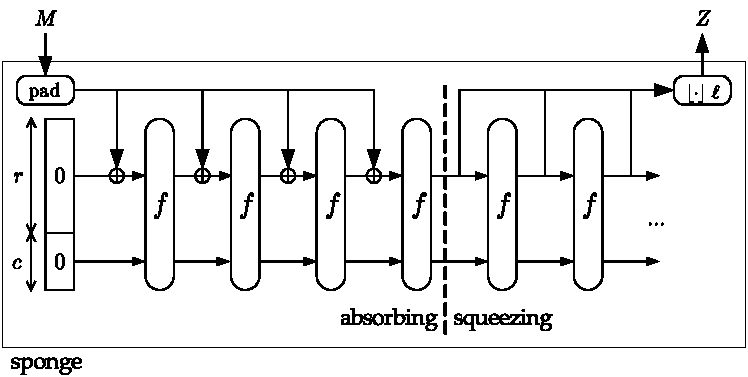
\includegraphics[scale=0.75]{sponge}
    \caption{Uma construção esponja. Imagem retirada de \cite{CSF}.}
    \label{fig:sponge}
\end{figure}

\begin{figure}[H]
    \begin{subfigure}{.5\textwidth}
        \centering
        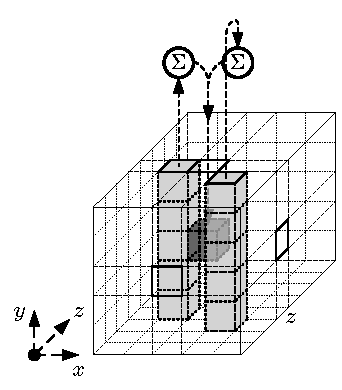
\includegraphics[scale=0.8]{theta_step}
    \end{subfigure}%
    \begin{subfigure}{.5\textwidth}
        \centering
        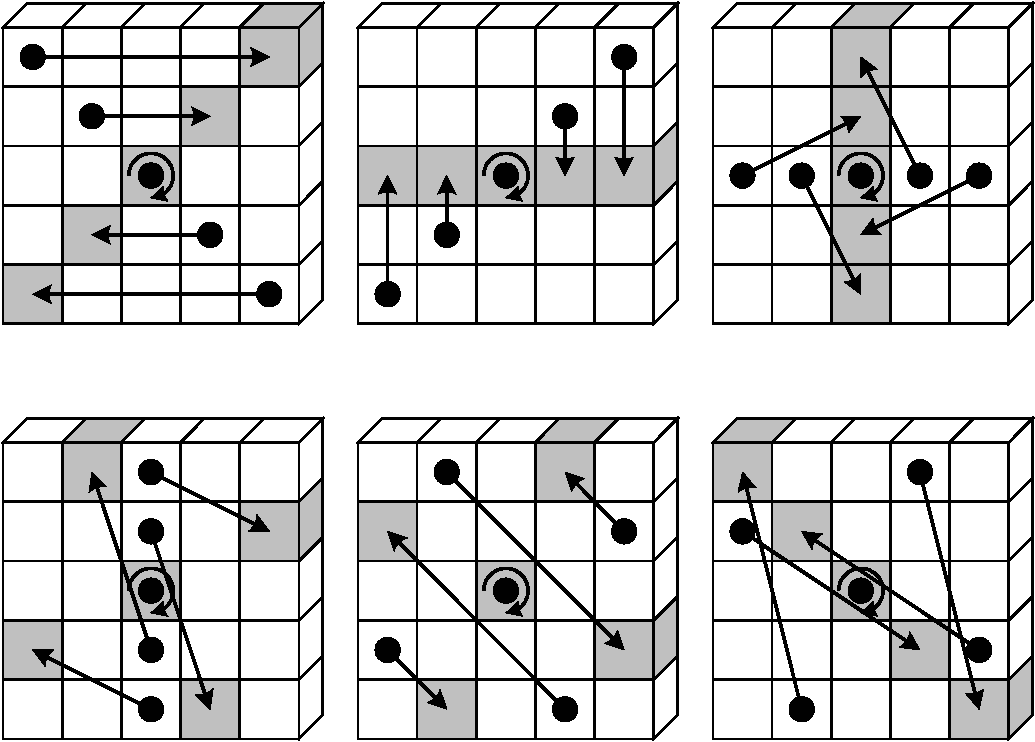
\includegraphics[scale=0.35]{pi_step}
    \end{subfigure}
    \begin{subfigure}{.5\textwidth}
        \centering
        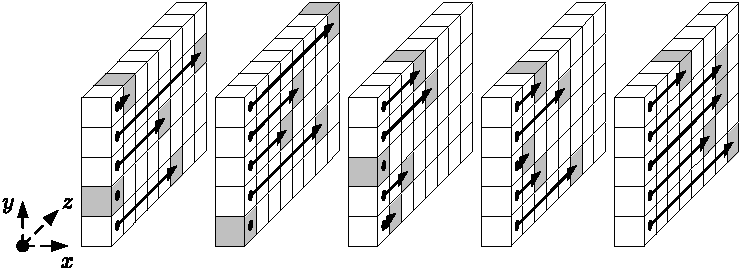
\includegraphics[scale=0.8]{rho_step}
    \end{subfigure}%
    \begin{subfigure}{.5\textwidth}
        \centering
        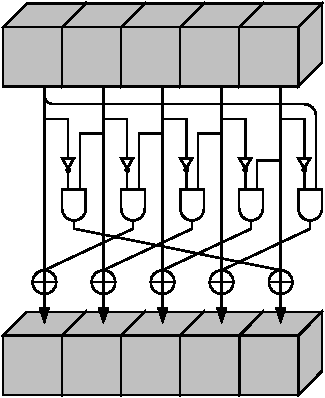
\includegraphics[scale=0.7]{chi_step}
    \end{subfigure}
    \caption{Da esquerda para a direita e de cima para baixo, as etapas
    $\theta$, $\pi$, $\rho$ e $\chi$. Imagens retiradas de
    \cite{KeccakReference}.}
    \label{fig:steps}
\end{figure}

\begin{itemize}

\item A etapa $\theta$ faz a soma \texttt{XOR} de uma elemento de $A$ e todos os
elementos das colunas adjacentes indicadas.

\item A etapa $\rho$ dispersa os elementos entre cortes transversais verticais
de $A$.

\item A etapa $\pi$ rearranja as posições de elementos em cortes transversais
horizontais de $A$.

\item A etapa $\chi$ tem como efeito fazer a soma \texttt{XOR} de cada bit em
uma linha, de acordo com uma função não-linear de dois outros bits adjacentes.

\item A etapa $\iota$ é utilizada para quebrar a simetria das operações acima,
e sem esta etapa, todas as rodadas teriam a mesma saída. A soma \texttt{XOR} de
alguns bits do estado $A$ é feita com um bit específico de uma sequência gerada
por um LFSR\footnote{\emph{linear-feedback shift register}, um tipo de gerador
de sequências pseudoaleatórias.}, alimentado pelo índice da rodada atual.

\end{itemize}

\end{itemize}

\bibliography{ine5429_t6}
\bibliographystyle{plain}

\end{document}
